\documentclass[a4paper,11pt]{article}
\usepackage{graphicx}
\usepackage[utf8]{inputenc}
\usepackage{hyperref}
\usepackage{placeins}
\usepackage[newfloat]{minted}
\usepackage{caption}

\newenvironment{code}{\captionsetup{type=listing}}{}
\SetupFloatingEnvironment{listing}{name=Code Overview}


\hypersetup{
    colorlinks=true,
    linkcolor=blue,
    filecolor=black,      
    urlcolor=blue,
    citecolor=black,
}
\begin{document}

\title{
    \textbf{Trees Report.}
}
\author{Adrian Jonsson Sjödin}
\date{Fall 2022}

\maketitle

\section*{Introduction}
In this assignment we will take a closer look at \textit{tree} structures, and in
particular at tree structure called \textit{binary trees}. The operations that we will look at and
implement are: construction, adding and searching for and removing an item.

\section*{Task}
Implement a binary tree structure that is ordered with smaller keys to the left and create the
following two methods:
\begin{itemize}
    \item {\tt add(Integer key, Integer value)}: adds a new node (leaf) to the
          tree that maps the key to the value. If the key is already present we
          update the value of the node.
    \item {\tt lookup(Integer key)}: find and return the value associate to the
          key. If the key is not found we return null.
\end{itemize}
benchmark the lookup algorithm and compare it to the benchmark of the binary search algorithm that
was done in a previous assignment.

Also create an iterator that we can use to traverse the tree. The iterator should implements Java's
Iterator class and override the {\tt hasNext()} and {\tt next()} method. Explain how you implemented
the methods of the tree iterator class. Also describe what will happen if you create an iterator,
retrieve a few elements snd then add new elements to the tree. Will it work, what is the state of the
iterator, will we lose values?

\section*{Method \& Theory}
This data structure is called a \textit{tree} since the structure originates in a root from where we
spread out into branches, that then in turn can further divide into their own branches. A branch that
does not divide further is terminated by a so called leaf.

A \textit{binary tree} is a tree whose branch always divides into two branches, unless it terminates
into a leaf.

I won't show the code for how the {\tt BinaryTree} class is constructed here since it
is already explained in the assignment, I will instead focus on the {\tt add()} and
    {\tt lookup()} method. When we create a Binary Tree we initialize it empty, i.e. the
root is set to null. The first node we add to the tree will then become the root, and
all subsequent nodes will then be added recursively down left or right of the root
depending on the node's key. If the key-value pair we want to add already exists in the
tree we instead change the value of that key-value pair to the new value. This ensures
that all key-value pairs are unique. Code overview \ref{code:add} shows how this work.

The {\tt lookup()} method however is not recursive, instead it uses a while loop to look
at each node, see if it is the key we want and if not go down left or right in the tree
depending on the current node's key size. It does this until we find the key we are looking
for, or we reach a null pointer in which case the key we're looking for doesn't exist in
the tree. This way of searching should give us a time complexity of $\mathcal{O}(h)$ where
$h$ is the height of tree. For a balanced tree (the height difference of nodes on
left and right subtree is not more than one) the height becomes $log(n)$, where $n$ is
the number of nodes in the tree. That means we should see a time complexity of
$\mathcal{O}(log(n))$ in our benchmark of the {\tt lookup()} method.




\section*{Result}
The result from the benchmark of the {\tt lookup()} method can be seen in figure \ref{fig:bench}.
In it we measure how long one long it takes to search for one random key from a tree
populated by $\sim4,000,000$ million random keys, and double the size of the tree for every measurement.
\begin{figure}[h]
    \centering
    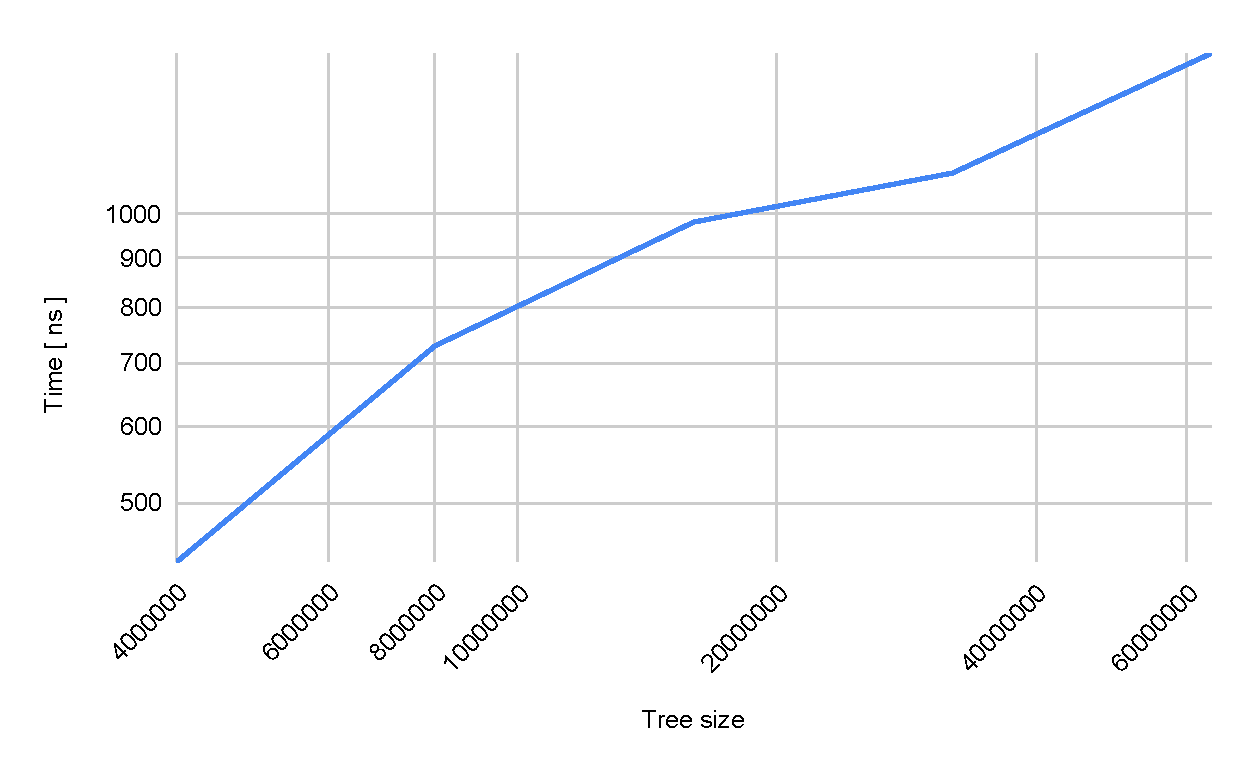
\includegraphics[width=.8\textwidth]{benchmarkData.pdf}
    \caption{Benchmark data for the {\tt lookup()} method}
    \label{fig:bench}
\end{figure}
\section*{Discussion}
As seen in figure \ref{fig:bench} the graph is somewhat linear in a log-log scale, which
indicates that our statement above about it being of time complexity $\mathcal{O}l(og(n))$.
The reason why the graph is somewhat skewed and not quite linear is probably because
in each benchmark a new tree with random branches are created and we're searching for a
random key. That means it is possible for some measurements to be faster if
we're lucky and the key we are searching for is closer to the root, than it is in a smaller
tree which then will take longer to search. With this in mind I feel that the data is
confirming my statement about the time complexity.

\newpage
\FloatBarrier
\section*{Code}
All the code can be found here: \href{https://github.com/adrian-jonsson-sjoedin/ID1021-AlgoData/tree/main/Tasks/Trees/src}{GitHub}

\begin{code}
    \captionof{listing}{Add to Binary Tree}
    \label{code:add}
    \begin{minted}{java}
public void add(Integer k, Integer v) {
    if (root == null) {
        root = new Node(k, v);
    } else {
        root.add(k, v);
    }
}        
private void add(Integer k, Integer v) {
if (this.key == k) {
    this.value = v;
}
if (this.key > k) {
    if (this.left == null) {
        this.left = new Node(k, v);
    } else {
        this.left.add(k, v);
    }
} else {
    if (this.right == null) {
        this.right = new Node(k, v);
    } else {
        this.right.add(k, v);
    }
}
}
\end{minted}
\end{code}

\end{document}
